%========================================================================================
% Compilation should work with PDFLaTeX
%========================================================================================
% Type of document and general formatting
\documentclass[a4paper,11pt]{article}

\usepackage[left=2.5cm,right=2.5cm,top=2.5cm,bottom=2.5cm]{geometry}
\linespread{1.25}

%========================================================================================
% These packages are for language and font settings
\usepackage[english,activeacute]{babel} % Language
\usepackage[T1]{fontenc}				% T1 Encoding of font
\usepackage[utf8]{inputenc}				% Special symbols
\usepackage{tgpagella}					% Text font


%========================================================================================
\usepackage[sc]{mathpazo}				% Math font
\usepackage{amsmath,amsfonts,amssymb}	% Math symbols
\usepackage{dsfont}						% Math symbols like R for reals...


%========================================================================================
% Other packages
\usepackage{graphicx}
\usepackage{longtable}
\usepackage[svgnames]{xcolor}

\usepackage{hyperref}
\hypersetup
{
    pdfauthor={Rafael Serrano-Quintero},
    pdfsubject={Matlab Notes},
    colorlinks = {true},
    linkcolor = {FireBrick},
    citecolor = {FireBrick},
    urlcolor = {RoyalBlue},
}

\usepackage{appendix}
\usepackage{marvosym}
\usepackage{enumerate} %For enumerating with letters with option [a)]
\usepackage{fancyvrb}  %To reduce font size in verbatim environment
\usepackage{epstopdf}
\usepackage[flushleft]{threeparttable}
\usepackage{natbib}
\usepackage{subcaption}
\usepackage{booktabs}
\usepackage[super]{nth}
\usepackage{float}
\usepackage{blindtext}		% Loren ipsum stuff


\newcommand{\source}[1]{\caption*{\tiny Source: {#1}} }

\newtheorem{exercise}{Exercise}
\newtheorem{remark}{Remark}

%========================================================================================
%========================================================================================
					% === Title, thanks, and author data === %
%========================================================================================
%========================================================================================


\title{\textbf{QED Macroeconomics III: Matlab Notes}}

\author{Rafael Serrano Quintero
\thanks{Department of Fundamentos del An{\'a}lisis Econ{\'o}mico, Universidad de Alicante. Email: \href{mailto:r.serrano@ua.es}{r.serrano@ua.es}} \\
Universidad de Alicante \\}
\date{\nth{3} Quarter 2018}


\begin{document}

\VerbatimFootnotes

\maketitle

\section{Getting Started}

Matlab is kind of a super calculator but also a programming language. You will be using it throughout the course to solve macroeconomic models, perform statistical analyses on macro variables, and most likely you will be using it in the future if you continue with macroeconomics. The name comes from \textit{Matrix Laboratory} and, as the name says, it is most useful to work with matrices, actually, you should try to \textit{vectorize} your codes as much as possible to enhance efficiency of your programs. To \textit{vectorize} means writing the operations of the code with matrix form as much as possible, sometimes you just cannot. This is because Matlab was actually optimized to use matrices, so use this on your behalf!

The starting screen of Matlab changes depending on the Matlab version and the user's configuration but usually, it looks like this:

\begin{figure}[htbp]
\centering
	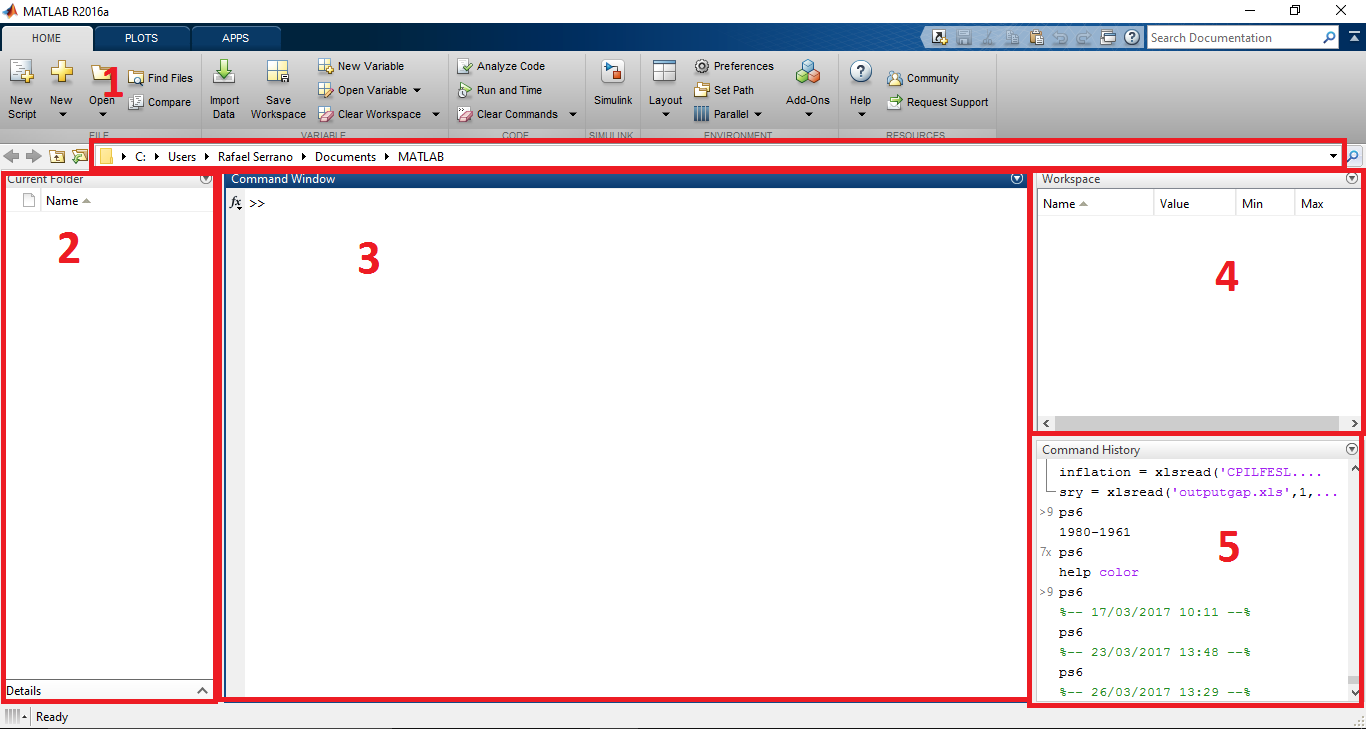
\includegraphics[width = 0.95\textwidth]{matlab_initial.png}
	\caption{Matlab's starting screen}
\end{figure}

\begin{enumerate}
	\item First box shows the \textbf{working directory}. This is the directory in your computer where Matlab will be working on.
	\item Second box shows the files in the current working directory. This is useful if we have several Matlab files, databases... that we will use in our task.
	\item The third box is the \textbf{command window}. Here you can type the commands you want Matlab to perform and the output will be displayed there.
	\item The fourth box is the \textbf{workspace}. Here Matlab will show the variables we have created. There can be different types of objects, matrices, cells, arrays... We will see them along the course.
	\item The fifth box is the \textbf{command history}. Here you can check the commands you have used already. It is useful if you want to repeat the same operation. \textit{\underline{Tip:} If you use the upper arrow key ($\uparrow$) in the command window, you will get access to the last command you used saved in the command history.}
\end{enumerate}

First of all, we should decide \textit{where} we will be working. I recommend you to be \textbf{very} organized when coding, because after a while, you won't remember all the details. So, first, create a new folder in which we will be working, let's name it \textbf{First Matlab Class} for example, this is done as usual (I assume you use Windows, but it's the same for Mac or Linux). Now, copy the directory for this file and paste it on the \textbf{working directory} in Matlab's main screen box 1.

In my case, this directory is:

\begin{Verbatim}[fontsize = \small]
D:\Dropbox\TEACHING\Master Macroeconomics III 2017-2018\1st Class Codes
\end{Verbatim}

Before we start working, let's introduce the first and most important function of Matlab. \verb;help;. Get familiar with this function by checking out some of the useful functions we will use:

\begin{Verbatim}[numbers = left,fontsize=\small]
help cd
help zeros
help eye
help ones
help randn
\end{Verbatim}

\section{Script versus Command Window}

We have said that in the command window we can type the commands we will want to use and the output will be shown there as well. However, this is not a useful way of using Matlab if we have longer tasks. To write down a proper assignment, we will use something similar to \textit{do-files} in Stata, a \textbf{script}. A script is a file that contains different lines of code in which each line performs a particular task. It is useful to write everything down in a script so that we can keep track of what we have done before and \textbf{correct mistakes} as we write our code. Matlab saves scripts with the file extension \verb;.m;.

To start a script in Matlab, you can do so by pressing the upper-left corner button \textit{``New Script''} or by typing in the command window \verb;edit;. A new window will open up and it should look something like Figure \ref{script}.

\begin{figure}
\centering
	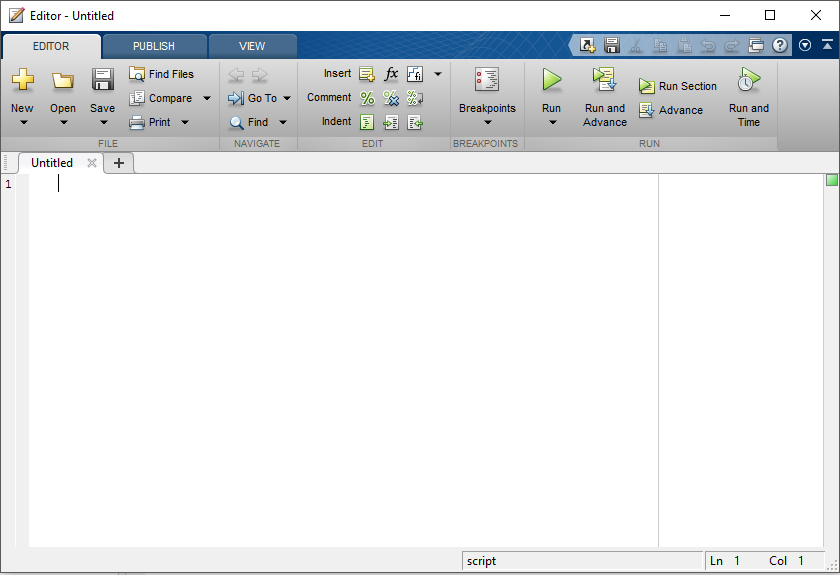
\includegraphics[width = 0.95\textwidth]{script1.png}
	\caption{Empty Matlab Script}
	\label{script}
\end{figure} 

These scripts are also very useful because we can write down comments in there just by using the symbol \verb;\%;. If we write that symbol, everything that is written after \textbf{in the same line} will not be interpreted by Matlab and will skip it. Another useful thing, are \textit{blocks of comments}. You can start a block of comments by using \verb;%{; and closing the block by using \verb;%};. Try to write as many comments so that you remember every detail of the operations you performed.

When programming it is important to follow some \textit{``rules''}. Here you have some suggestions that will make life easier. 

\begin{enumerate}
	\item \textbf{Clever is the enemy of clear}: aim for clarity, not efficiency. A code should be clear first of all so everyone understands what you're doing and how. The simpler, the better. Sometimes you can solve a problem with a couple lines of code, but it might be very difficult to know what the code is doing, it is better to add some more lines if this helps understand what's going on.
	\item \textbf{Write code if and only if you have to:} this does NOT mean you should write the code as compact as you can, but that you should write the code that solves the problem you're interested in and, if you can, use the functions that already exist. This saves time and helps to understand the way in which you obtain your results.
	\item \textbf{Test your code before sending it:} the code should work and be self-contained. That means it should be as simple as running it to get the desired results. Suppose you write a code to solve a problem, but you need to run a different code first or use a function, you should provide the additional codes and call them right in the script.
	\item \textbf{Self-documented codes:} start your code by providing a brief explanation of what the code is intended to do, provide short comments when the code is not self-explanatory, use variable names that helps you know what that variable is...
\end{enumerate}

\section{Creating Variables}

Matlab deals with several types of objects, we will start by using mostly matrices (even if we assign to a variable just a number, this is interpreted as a matrix $1\times 1$). There exist other types such as \textit{strings} (text characters), complex numbers, symbolic variables...

To name a variable, the first character \textbf{needs} to be a letter, after that, any combination is allowed. Matlab is case sensitive (it is not the same $x$ or $X$). Some names should not be used because they already indicate something in Matlab:

\begin{itemize}
	\item $i$ and $j$ can indicate complex numbers.
	\item \verb;pi; is assigned to $\pi$.
	\item \verb;ans; is assigned to the last value that has not been assigned to anything.
	\item \verb;Inf; or \verb;-Inf; are positive and negative $\infty$.
	\item \verb;NaN; represents \textbf{``Not a Number''}.
	\item \verb;eps; is designated to be the \textit{machine epsilon} (we will comment a bit on this below).
\end{itemize}

We define a variable $x$ to have the value $5$ as:

\begin{Verbatim}[numbers=left]
x = 5;
\end{Verbatim}

Notice the semicolon (\verb+;+) at the end, this is to suppress output. Now that the variable $x$ has been assigned to a value, we can construct a function out of it. For example, suppose we want to construct another variable $y = x^2$, this is done simply by:

\begin{Verbatim}[numbers=left]
y = x.^2
\end{Verbatim}

The dot right before the \verb+^+ indicates that this is an \textbf{element-wise} operation. That is, it applies the squaring to \textit{each} element in $x$. In our case, $x$ has only one element.

\begin{exercise} 
Use Matlab as a calculator and try to solve the following operations using the functions needed. Solve them for $x = 0$ and $x = \frac{\pi}{4}$

\[
		\frac{\left(\ln\big( 1+x^2\big)\right)^2 - \sqrt{1+\sqrt[3]{x^2}\,}}{1+\sin^2 x} \ ; \  \ln\bigg\lvert\frac{x-\pi}{x+\pi}\bigg\rvert + \sqrt{\frac{e^x}{1+xe^x}}
\]
\end{exercise}

\textbf{Check the commands:}
\begin{itemize}
	\item \verb+log+
	\item \verb+sqrt+
	\item \verb+sin+
	\item \verb+exp+
	\item \verb+abs+
\end{itemize}

A useful resource provided by \textit{Quant-Econ} is this \href{https://cheatsheets.quantecon.org/}{{\textbf{Cheat-Sheet}}}.

\section{Vectors}

To create a \textbf{row vector}:

\begin{Verbatim}[numbers=left]
rowV = [1 2 3 4 5];
rowV2 = [6, 7, 8, 9, 10];
\end{Verbatim}

To create a \textbf{column vector}:

\begin{Verbatim}[numbers=left]
colV = [1; 2; 3; 4; 5];
\end{Verbatim}

\textit{\underline{Suggestion:} Check your workspace!!}

To check sizes and lengths of vectors, commands \verb+size+ and \verb+length+ are available. There are other useful commands to create vectors, check what is the difference between the following two sequences.

\begin{Verbatim}[numbers = left]
seq1 = 0:10;
seq2 = linspace(0,10,1000);
\end{Verbatim}

\section{Matrices}

Matrices can be created element by element or by concatenating vectors. A space between two elements indicates they're in the same row, a semicolon (;) after a number indicates that is the last element of the row.

Matrix transpose can be computed either by using \verb+transpose()+ or by using the operator \verb+'+ at the end of the matrix's name.

To compute an inverse, we can use \verb+inv()+ command.

To perform operations with matrices, we can use either element-wise operations or regular matrix operations. To illustrate, consider two matrices:

\[
A = \begin{bmatrix}
1 & 2 & 3 \\
4 & 5 & 6 \\
7 & 8 & 9 
\end{bmatrix} \ ; \ 
B = \begin{bmatrix}
4 & 5 & 6 \\
7 & 9 & 2 \\
1 & 5 & 32
\end{bmatrix}
\]

Element-wise product, for example, would mean computing  $a_{i,j} \times b_{i,j}$ where $a_{i,j}$ denotes the $ij-$th element of matrix $A$ and $b_{i,j}$ denotes the $ij-$th element of matrix $B$. So, in this case, element-wise multiplication would yield:

\[
A \odot B = 
\begin{bmatrix}
     4  &  10 &   18 \\
    28  &  45 &   12 \\
     7  &  40 &  288
\end{bmatrix}
\]

Instead, regular matrix product would yield:

\[
AB = 
\begin{bmatrix}
  21  & 38 &  106 \\
  57  & 95 &  226 \\
  93  & 152 &  346
\end{bmatrix}
\]

Be careful with element-wise operations, with matrices, sizes of $A$ and $B$ should be the same, but what do you think would happen if we multiply \verb+rowV.*rowV2'+?. To perform matrix operations, it will depend on the operation itself. Matrix products need the inner dimensions to be the same, that is, if $A$ and $B$ are two matrices of sizes $(m\times n)$ and $(j \times k)$, then to be able to multiply them, we need $n = j$. Matrix exponentiation needs square matrices. Matrix division needs that the inverse exists. In Matlab, element-wise operations are performed by adding a dot $(.)$ before the operator.

\begin{itemize}
	\item Element-wise operations:
	\begin{itemize}
		\item Product \verb+.*+
		\item Exponentiation \verb+.^+
		\item Division \verb+./+		
	\end{itemize}
	\item Standard matrix operations:
	\begin{itemize}
		\item Product \verb;*;
		\item Exponentiation \verb;^;
		\item Left or right division \verb;/\; (\verb;mldivide; is equivalent)
	\end{itemize}
\end{itemize}

The left division is usually defined as $A \backslash B = A^{-1} B$ and the right division is usually defined as $ A / B = AB^{-1}$. To avoid any confusions, I prefer to pre- or post-multiply by the inverse of the matrix I need, as long as the matrix is small and \textit{``well-behaved''}. Note that left division needs that the inverse of $A$ exists and right division needs that the inverse of $B$ exists. However, the procedure of actually using command \verb;inv(); might not give the best result for larger matrices. To solve systems of equations, \textbf{it is recommended to use} the \verb;\; operator (this operator actually uses Gaussian elimination, check \verb;help \; to see how this operator also solves over- or underdetermined systems). 

\begin{exercise} 
Solve the following system of linear equations using \verb;inv(); and \verb;\;.

\begin{alignat*}{7}
3x&& \; + \; &&2y&& \; - \; &&z&& \; = \; &&1&\\
2x&& \; - \; &&2y&& \; + \; &&4z&& \; = \; &&-2&\\
-x&& \; + \; &&{\tfrac {1}{2}}y&& \; - \; &&z&& \; = \; &&0&
\end{alignat*}
\end{exercise}

\subsection{Accessing Elements of a Matrix}

There will be occasions that we will want to take subsets of matrices and Matlab allows us to access elements of matrices in a convenient way. Suppose you want to access columns 2 to 5 of a matrix $A$ keeping all the rows, that is as simple as typing \verb;A(:,2:5);. The bracket indicates we are accessing matrix $A$, the first element inside the bracket denotes the first dimension of matrix $A$ (rows) and the second denotes columns. Two dots (\verb;:;) denotes \textbf{all} the elements in that dimension. The \verb;2:5; indicates we are choosing elements $2$ to $5$ in steps of 1, and , because it is in the column dimension, it tells Matlab to take those columns.

To know the dimensions of a matrix, you can use \verb;size();. This command gives back a vector in which the first element is the number of rows of the matrix and the second the number of columns (you can also use it with $n$-dimensional arrays). Try to play around with subsetting elements of the array \verb;M = randn(10,3,5); and try to understand its shape.

\subsection{Wonkish Remark on Invertibility and Matlab}

\textit{This is not necessary right now but it might be useful in the future, skip it for now if you're not very interested.}

To test whether a matrix is invertible, a possibility is to use its condition number\footnote{This is usually defined as \[cond(A) = \left\lVert A \right\rVert \cdot \left\lVert A^{-1} \right\rVert = \frac{\lambda_{max}}{\lambda_{min}}\] which is the ratio of the maximum stretching to the minimum stretching a matrix does to any non-zero vector. If the condition number is large, it means the matrix is nearly singular. Last equality applies if $A$ is normal. A matrix is normal if and only if it is unitarily similar to a diagonal matrix.} with respect to the inverse (\verb;cond(); in Matlab), this will give us some indication of the accuracy of the results from matrix inversion and the linear equation solution. A rough threshold for the condition number can be the one used by Matlab, $cond(\mathbf{A}) < 1/((max(size(\mathbf{A}))\varepsilon)$ where $\mathbf{A}$ is a matrix and $\varepsilon$ is the machine epsilon used by Matlab\footnote{The machine epsilon in Matlab is \verb;2.2204e-16; roughly means that numbers are stored with about 15-16 digits of precision. If a number is approximately 1, then that means it can be stored with an error of around \verb;10^(-16); or so, the command to use this machine epsilon is \verb;eps; in Matlab.}. To see why this can be useful, suppose we have an identity matrix of size $15$ multiplied by $0.0001$, this matrix is non-singular because it is based on the identity matrix. However, try computing the determinant.

\begin{Verbatim}[numbers=left]
A = 0.0001 * eye(15);
det(A)
ans =
   1.0000e-60
\end{Verbatim}

It is very close to zero but still it is well conditioned. An example in which the function \verb+det()+ does not work is the following large singular matrix (it is singular because the sum of all rows yields the null vector). Suppose the matrix is:

\begin{verbatim}
 24   -13    0      0     0     0     0     0     0     0     0     0     0
-24    46   -24     0     0     0     0     0     0     0     0     0     0
 0    -33    64   -33     0     0     0     0     0     0     0     0     0
 0     0    -40    78   -40     0     0     0     0     0     0     0     0
 0     0     0    -45    88   -45     0     0     0     0     0     0     0
 0     0     0     0    -48    94   -48     0     0     0     0     0     0
 0     0     0     0     0    -49    96   -49     0     0     0     0     0
 0     0     0     0     0     0    -48    94   -48     0     0     0     0
 0     0     0     0     0     0     0    -45    88   -45     0     0     0
 0     0     0     0     0     0     0     0    -40    78   -40     0     0
 0     0     0     0     0     0     0     0     0    -33    64   -33     0
 0     0     0     0     0     0     0     0     0     0    -24    46   -24
 0     0     0     0     0     0     0     0     0     0     0    -13    24
\end{verbatim}

Computing the determinant using \verb;det(); yields as a result \verb;1.0597e+05; when in fact it should be 0. However, if we compute the condition number, this is very large indicating the matrix is ill-conditioned (\verb;cond() = 5.7306e+16;).

To extract elements of matrices, it is as simple as using parentheses and typing the element you need. If we want the element in the first row and second column of matrix $A$, we would type in Matlab \verb;A(1,2);, if we want a whole column or row, we use the colon operator \verb;:;.


\begin{remark}

\textbf{Why \textbackslash is superior to \texttt{inv(A)*b} to solve systems of equations:}\footnote{Taken from \url{es.mathworks.com/help/matlab/ref/inv.html}} Create a random matrix A of order $500$ that is constructed so that its condition number, \texttt{cond(A)}, is \texttt{1e10}, and its norm, \texttt{norm(A)}, is 1. The exact solution $x$ is a random vector of length $500$, and the right side is $b = Ax$. Thus the system of linear equations is badly conditioned, but consistent (there is at least one set of values for $x$ that satisfy each of the equations). 

\begin{Verbatim}[numbers=left]
n = 500; 
Q = orth(randn(n,n));
d = logspace(0,-10,n);
A = Q*diag(d)*Q';
x = randn(n,1);
b = A*x;

y1 = inv(A)*b; 
y2 = A\b;

res_inv = norm(A*y1-b)
res_bs = norm(A*y2-b)
\end{Verbatim}

To see this, the eigenvalues of $A$ are given by the diagonal entries of $d$ because $A$ is orthogonally diagonalizable, the condition number can be expressed as $cond(A) = \frac{\lambda_{max}}{\lambda_{min}}$ (because $A$ is normal) and, in this case, by construction, it is $cond(A) = 1/10^{-10} = 10^{10}$. So the condition number is very large but the inverse of $A$ exists. The residuals are larger for the case in which we compute the solution using \texttt{inv} because it does not use Gaussian elimination and the rounding errors are much larger.
\end{remark}

\section{Simple Plots}

In Matlab we can do nice plots easily. You can either plot a variable against its own index or plot a variable against some other values. The important is that both variables are the same size.

Suppose we want to plot a particular function, for example, $sin(x)$. What we can do is define a domain for $x$ by using either some automated method or creating a vector by ourselves and then, define another variable that corresponds to the function we want to plot.

As an example, suppose that we want to plot both $sin(x)$ and $cos(x)$, the following code will do the trick:

\begin{Verbatim}[numbers=left]
x = linspace(0,3*pi,10000);
y = sin(x);
g = cos(x);

figure
plot(x,y,'--','LineWidth',1.35)
hold on
grid on
plot(x,g,'-','LineWidth',1.35)
xlim([0 3*pi])
legend({'$\sin(x)$','$\cos(x)$'},'Interpreter','latex','Location','best')
title('Sine versus Cosine')
xlabel('$$x$$','Interpreter','latex')
ylabel('$$F(x)$$','Interpreter','latex')
\end{Verbatim}

This figure is a bit more complicated, but it shows the power of Matlab graphics, we can use \LaTeX\ within its graphic environment. The first line defines a vector of $10000$ evenly spaced points in the range $[0,3\pi]$. The second and third lines define two variables $y$ and $g$ corresponding to the $\sin(x)$ and $\cos(x)$. The fifth line simply tells Matlab that this will be a figure (you can omit that, but it is useful to write it down when you want to display several figures with just one code). The sixth line is the actual command for plotting. It plots $y$ as a function of $x$. The \texttt{'- -'} tells Matlab we want a discontinuous line and the \texttt{'LineWidth'} just indicates how thick we want the line to be. The \texttt{hold on} command tells Matlab the figure is not done yet and allows us to include other plots in the same figure, the function $g$ in this case. The rest are some additional fancy touches to make the graph look a bit more \textit{``professional''}.

\textit{\underline{Suggestion:} check all available functions that are useful for the } \texttt{plot} \textit{environment using} \texttt{help plot}.

Matlab also allows for 3D plots. In Figure \ref{3dscatter} you have a 3D scatterplot of the variables you will simulate in the Problem Set, do not worry very much about the details of the Figure, if you're interested we will see the code in class. Check commands \texttt{scatter3, meshgrid, mesh, plot3} and try to do some 3D plots yourself.

\begin{figure}
\centering
	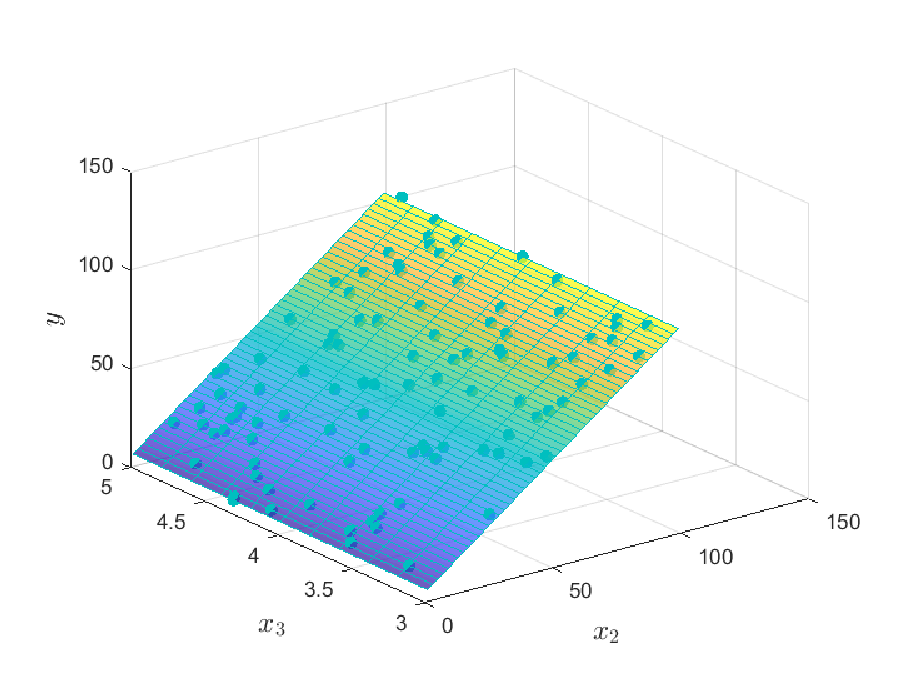
\includegraphics[width = 0.65\textwidth]{3dscatter.eps}
	\caption{3D Scatterplot}
	\label{3dscatter}
\end{figure}

\begin{exercise}
Plot in the \textbf{same} figure a simple sine wave with amplitude and frequency one, and a sine wave with amplitude four and frequency $\pi/2$. That is, plot $F(x)$ and $G(x)$:

\[
F(x) = sin(x) \ ; \ G(x) = 4sin(\tfrac{\pi}{2}x)
\]

Use $10000$ points for $x\in[0,10]$.
\end{exercise}

\section{Functions}

Even if Matlab has lots of built-in functions, we may want to define some of our own. That is, we can create files that perform a particular task we tell it to. It is important to note that functions need to be written in a \textbf{separate} file that will only contain that function. However, keep in mind that for Matlab to find the function, this needs to be saved in your working directory.

Suppose we are going to create our own function to compute the factorial of a number, Matlab already has a function that does this operation \texttt{factorial()} but this is useful for illustration and practice purposes. Recall that the factorial is defined as:

\[
n! = n\times(n-1)\times(n-2)\times \ldots 1 
\]

The important thing a user-defined function must have in Matlab is the declaration that it is a function. We do so by directly including the word \texttt{function}. The basic structure of any function in Matlab is:

\begin{Verbatim}[numbers=left]
function [Output Arguments] = F(Input arguments)
	Output Arguments = The operations we want to perform on the Input Arguments
end
\end{Verbatim}

So a code that would do for computing the factorial of any number $n$ would be:

\begin{Verbatim}[numbers=left]
function [output_arg] = my_factorial(n) 
	output_arg = prod(1:n)
end
\end{Verbatim}

Note that if we want to \textbf{use} this function, we can call it in the command window or in our script just as we use \verb;sin(); or any other function. However, we must save the file in the \textbf{same directory} we are currently working, otherwise, Matlab will not find the function and will display an error.

\begin{exercise}
Create a function called \verb;my_wave; that gives as output the plot of a sinusoidal wave. The function should take as arguments the parameters that will give the amplitude and the frequency, and the upper and lower bounds in which it will be plotted. By default, plot $10000$ points. Plot the sinusoidal wave with amplitude and frequency one for comparison.
\end{exercise}

\section{Loops and Conditionals}

Sometimes it is useful to repeat the same operation multiple times or repeat a task until some condition is met. Another useful thing is to perform some task \textit{if} something has happened, that is, perform a task conditioning on something happening. We can do all these things in Matlab by writing loops (cycles) and/or conditionals.

Suppose first you have a set of values for which you want to perform an operation. In this case, you may want to use a \textbf{for} loop. Let's suppose we want to create some vector that contains a sequence from 1 until a maximum $T$. A way to do so, is to write a loop such as:

\begin{Verbatim}[numbers=left]
for t=1:T
	Y(t,1) = t;
end
\end{Verbatim}

The for loop performs some task for all the indices that we declare. Another way to do so is by using a \textbf{while} loop. The difference between a \textbf{while} and a \textbf{for} loop is that the first performs the operation as long as a condition is fulfilled. The latter, will perform the operation for a fixed range of values or indices.

\begin{Verbatim}[numbers=left]
t = 1
while t<=T
	Y(t,1) = t
 	t = t+1
end
\end{Verbatim}

Note that for both the \texttt;for; and the \texttt;while; loops, what is written inside the loop appears indented. This is \textbf{not} necessary but you will see that it is useful to keep a clean and ordered code. The nice property of the \textbf{while} loop is that it will perform the iterations as long as a condition holds. This is useful if we want to do an operation until some convergence degree (precision). To state these conditions, Matlab uses \textbf{relational} and \textbf{logical} operators. The most common ones are:

\begin{itemize}
	\item Relational Operators:
	\begin{itemize}
		\item Equal \verb;==;
		\item Not equal \verb;~=;
		\item Greater than \verb;>; or Less than \verb;<;
		\item Greater or equal than \verb;>=; or less or equal than \verb;<=;
	\end{itemize}
	\item Logical Operators:
	\begin{itemize}
		\item And \verb;\&;
		\item Or \verb;|;
		\item Not \verb;~;
		\item All true \verb;all;
		\item Any true \verb;any;
	\end{itemize}
\end{itemize}

These operators will be useful to define \textbf{if/else/elseif} statements. These will be blocks of codes that if a condition holds, the block will perform some tasks. The most basic structure would be:

\begin{Verbatim}[numbers=left]
if Condition
	Commands
end
\end{Verbatim}

In this case, the commands execute \textbf{only if} the condition holds. We may want to add some commands in case the condition evaluates to False (that is the same as to say that the condition does not hold). To do so, we would include \verb;else; parts. The basic structure would be:

\begin{Verbatim}[numbers=left]
if condition
	Commands in case Condition is True
else
	Commands in case Condition is False
end	
\end{Verbatim}

We might also want to include two distinct conditions. That's when we can use \texttt;elseif;. A basic structure would be:

\begin{Verbatim}[numbers=left]
if Condition 1
	Commands in case Condition 1 is True
elseif Condition 2
	Commands in case Condition 2 is True
else
	Commands in case Conditions 1 and 2 are False
end
\end{Verbatim}

Note that all examples for loops and for conditionals are indented. This is useful when we have loops inside loops or conditionals inside loops.

\begin{exercise}
Suppose we have a list of grades of students. Create a loop that goes through all the notes and checks whether that student has passed the subject or not. To get the list, generate a random list of 200 grades uniformly distributed between 0 and 10 (check \verb;rand; command), and to assign if a student has passed or not, generate a vector called \verb;passed; that equals one if the student has obtained a grade larger or equal than 5, and 0 otherwise.
\end{exercise}

\begin{remark} 

\textbf{On Preallocation:} A typical use of \verb;for; and \verb;while; loops is that of creating iteratively a vector or a matrix. If with each iteration we increase the size of the particular vector, Matlab will require additional memory each time so the code will not be efficiently implemented. It is thus recommended that you \textit{pre-allocate} the necessary memory for that vector or matrix and change the values as iterations pass. 

As an example take previous exercise. We do not know how many students passed \textit{a priori} but we do know how many students there are in the list. To efficiently implement the code that will tell us which student passed and which failed, we could first create the vector of passed students, perform the loop and the conditionals, and change the values of the pre-allocated vector as we iterate over students. To do so, we could proceed as follows\footnote{To check this, you can try this example from \href{https://es.mathworks.com/help/matlab/matlab_prog/preallocating-arrays.html}{{Matlab's Documentation}}}
\end{remark}

\begin{Verbatim}[numbers=left]
passed = vector that takes values of 1 of the same length as the students' list.

for each student in the list
	if the student's grade is > 5
		passed takes 1 in the place of that student
	otherwise
		passed takes 0 in the place of that student
	end
end		
\end{Verbatim}

\section{Some Shortcuts and Tips}

Here are some tips and shortcuts you can use to work with Matlab for Windows, I do not use Mac or Linux so I have no idea, but probably they're very similar.

\begin{itemize}
	\item \verb;F9; (in some laptops as mine, you need to press also \verb;Fn;) allows you to run just a selected row or piece of code.
	\item \verb;Ctrl + C; in the command window allows you to stop any running code.
	\item \verb;Tab; when you start writing a function, if you press it, it will display the autocomplete suggestions.
	\item \verb;Ctrl + R; sets selected text to comments.
	\item \verb;Ctrl + N; opens a new script.
	\item \verb;whos; tells you information about the variables saved in your workspace.
	\item \verb;break; is a command that can be used to stop the code but should be used within the script. Suppose you are running a loop and you don't want to perform more than $1000$ iterations, you could set a conditional that if the maximum number of iterations is reached, then the whole code stops.
	\item \verb;disp(); is a command that allows you to display text in the command window.
	\item Note that with loops, it is easy to make mistakes and create infinite loops. To avoid that, if you have to do $1000$ iterations, start by doing first $10$ and do not write the \verb+;+ to see the output in the command window. If everything looks fine, then go for all the iterations.
	\item \verb;k:j:m; is a way of creating a vector from $k$ to $m$ in steps of $j$ before we were using \verb;k:m; that, by default sets $j=1$.
	\item Some other useful commands \verb;diag;, \verb;ones;, \verb;zeros;, \verb;eye;, \verb;reshape;, \verb;eig;, \verb;det; you can check them in Matlab's documentation.
\end{itemize}

\end{document}